\begin{figure}[htbp]
\centering
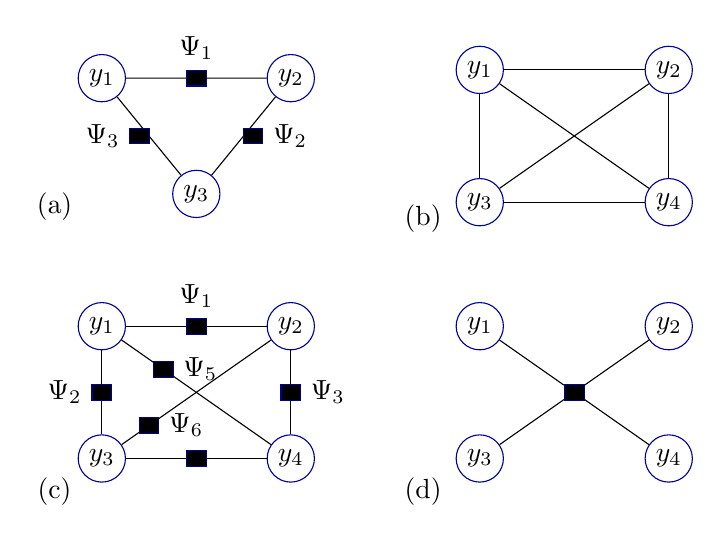
\begin{tikzpicture}[x=1.2cm,y=1.05cm,
chSixFtwelveV/.style={circle,draw=blue!60!black,fill=white,minimum size=6mm,inner sep=1pt},
chSixFtwelveF/.style={rectangle,fill=black,draw=blue!60!black,minimum width=2.5mm,minimum height=2mm,inner sep=0pt}]
\node[chSixFtwelveV] (chSixF12a1) at (0,4) {$y_1$};\node[chSixFtwelveV] (chSixF12a2) at (2,4) {$y_2$};\node[chSixFtwelveV] (chSixF12a3) at (1,2.6) {$y_3$};
\draw (chSixF12a1)--(chSixF12a2)--(chSixF12a3)--(chSixF12a1);
\node[chSixFtwelveF,label=above:$\Psi_1$] at (1,4) {};\node[chSixFtwelveF,label=right:$\Psi_2$] at (1.6,3.3) {};\node[chSixFtwelveF,label=left:$\Psi_3$] at (.4,3.3) {};
\node at (-.5,2.45) {(a)};
\foreach \nn/\xx/\yy in {1/4/4.1,2/6/4.1,3/4/2.5,4/6/2.5}
 \node[chSixFtwelveV] (chSixF12b\nn) at (\xx,\yy) {$y_{\nn}$};
\foreach \aa/\bb in {1/2,1/3,1/4,2/3,2/4,3/4} \draw (chSixF12b\aa)--(chSixF12b\bb);
\node at (3.4,2.3) {(b)};
\foreach \nn/\xx/\yy in {1/0/1,2/2/1,3/0/-.6,4/2/-.6}
 \node[chSixFtwelveV] (chSixF12c\nn) at (\xx,\yy) {$y_{\nn}$};
\foreach \aa/\bb in {1/2,1/3,1/4,2/3,2/4,3/4} \draw (chSixF12c\aa)--(chSixF12c\bb);
\node[chSixFtwelveF,label=above:$\Psi_1$] at (1,1) {};
\node[chSixFtwelveF,label=left:$\Psi_2$] at (0,.2) {};
\node[chSixFtwelveF,label=right:$\Psi_3$] at (2,.2) {};
\node[chSixFtwelveF] at (1,-.6) {};
\node[chSixFtwelveF,label=right:$\Psi_5$] at (.65,.48) {};
\node[chSixFtwelveF,label=right:$\Psi_6$] at (.5,-.2) {};
\node at (-.5,-1) {(c)};
\foreach \nn/\xx/\yy in {1/4/1,2/6/1,3/4/-.6,4/6/-.6}
 \node[chSixFtwelveV] (chSixF12d\nn) at (\xx,\yy) {$y_{\nn}$};
\node[chSixFtwelveF] (chSixF12df) at (5,.2) {};
\foreach \nn in {1,2,3,4} \draw (chSixF12d\nn)--(chSixF12df);
\node at (3.4,-1) {(d)};
\end{tikzpicture}
\origfig{12}{因子图。（a）三个变量上的因子图（引文见例 A1）；（b）具有完全连接图的马尔可夫随机场（引文见例 A2）；（c）该马尔可夫随机场的一种可能因子分解（引文见例 A2）；（d）一个因子图（引文见习题 5）。}
\end{figure}
